\documentclass{article}

% Language setting
% Replace `english' with e.g. `spanish' to change the document language
\usepackage[T2A]{fontenc}
\usepackage[utf8]{inputenc}

% Set page size and margins
% Replace `letterpaper' with `a4paper' for UK/EU standard size
\usepackage[letterpaper,top=2cm,bottom=2cm,left=3cm,right=3cm,marginparwidth=1.75cm]{geometry}

% Useful packages
\usepackage{amsmath}
\usepackage{graphicx}
\usepackage{float}
\usepackage[colorlinks=true, allcolors=blue]{hyperref}

\title{Лабораторная работа №1}
\author{Выполнили: Цалов В.С.}

\begin{document}
\maketitle
Преподователь: Оранский С.И.

\title{Вариант 4}

\section{Задание №1}
\subsection{Выбранное распределение}

В качестве распределения было выбрано распределение хи-квадрат.
Плотность распределения будет здесь может быть

Гистограмма этого распеределения выглядит примерно так:

\begin{center}
      \centering
      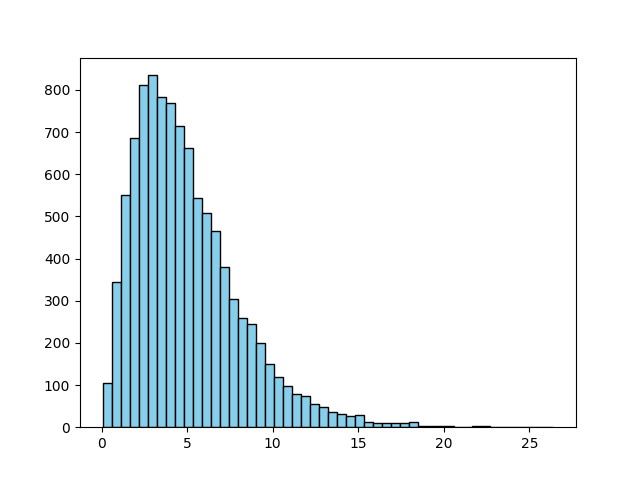
\includegraphics[width=0.5\linewidth]{Python/chi.png}
\end{center}

\subsection{Первый эксперемент}
В ходе данного задания были проведен эксперемент в ходе которого были созданы 10 000 выборок по 1000 значений данного распеределения.
в этих выборках были подсчитаны: среднее выборочное значение, выборочная дисперсия и выборочный квантиль поярдка 0.5 (медиана выборки) 

Гистограммы этих значений
\begin{figure}[H]
      \centering
      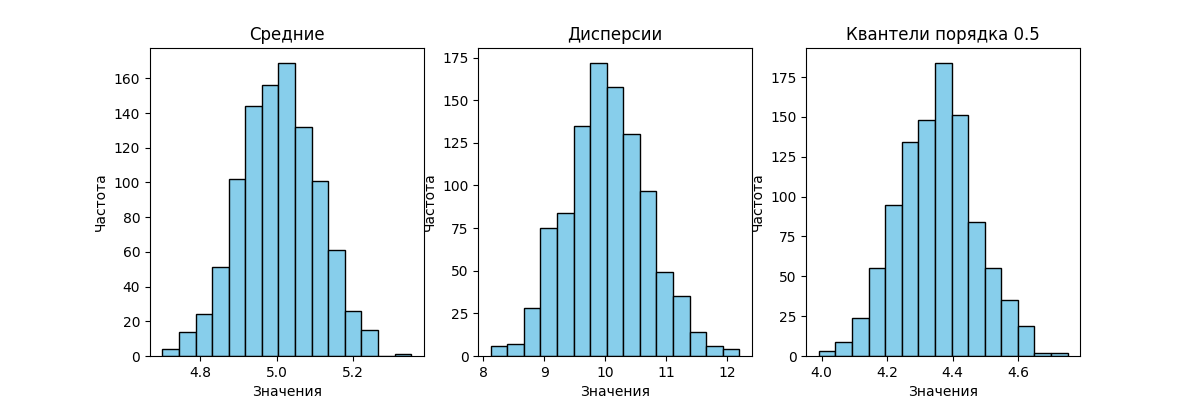
\includegraphics[width=0.8\linewidth]{Python/first-exp.png}
      \caption{Гистограммы параметров выборки}
\end{figure}
% \begin{center}
%       \begin{figure}
%             \centering
%             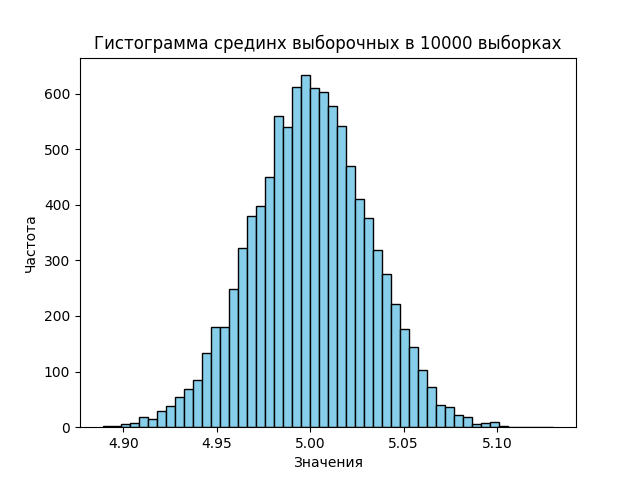
\includegraphics[width=0.5\linewidth]{Python/hist-mean.png}
%             \caption{Среднее выборочное значение для всех выборок}
%       \end{figure}
%       \begin{figure}
%             \centering
%             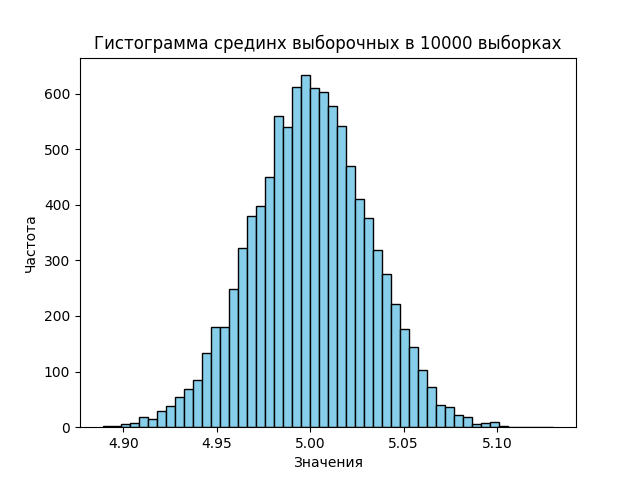
\includegraphics[width=0.5\linewidth]{Python/hist-mean.png}
%             \caption{Среднее выборочное значение для всех выборок}
%       \end{figure}
%       \begin{figure}
%             \centering
%             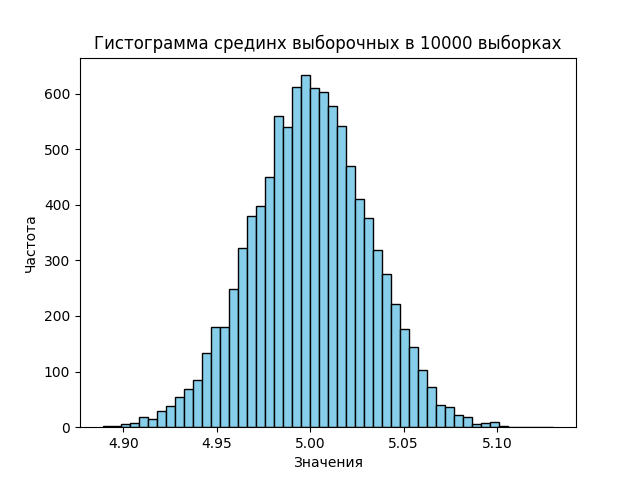
\includegraphics[width=0.5\linewidth]{Python/hist-mean.png}
%             \caption{Среднее выборочное значение для всех выборок}
%       \end{figure}
% \end{center}

\subsection{Вывод по первыой части}
Можно заметить, что данные выборки представляют собой нормальное распеределение, что подтвержадется центральной передельной теоремой, которая гласит: бла бла бла


\subsection{Сравнение с Гамма-распределением}
Второй эксперемент заключается в том, что нам надо сравнить порядковые статистки с гамма-распределением.
Сортируем каждую выборку для нахождения второй и n-ой порядковой статистики $F(X_{(2)}$ и $F(X_{(n)})$.
Затем находим значения $nF(X_{(2)}$ и $n(1 - F(X_{(n)}))$ и затем заносим их в выборку.
Далее генерируем гамма распределение с параметрами $\Gamma(2, 1)$ и $\Gamma(1, 1)$

В итоге получаем такие графики:

\begin{figure}[H]
      \centering
      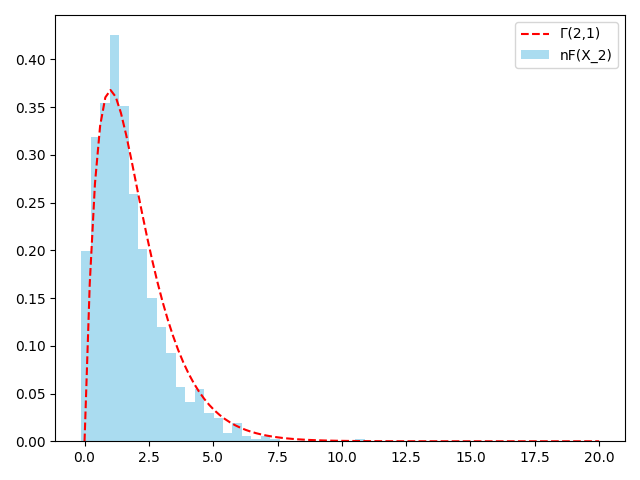
\includegraphics[width=0.5\linewidth]{Python/second-two-one.png}
      % \caption{}
\end{figure}
\begin{figure}[H]
      \centering
      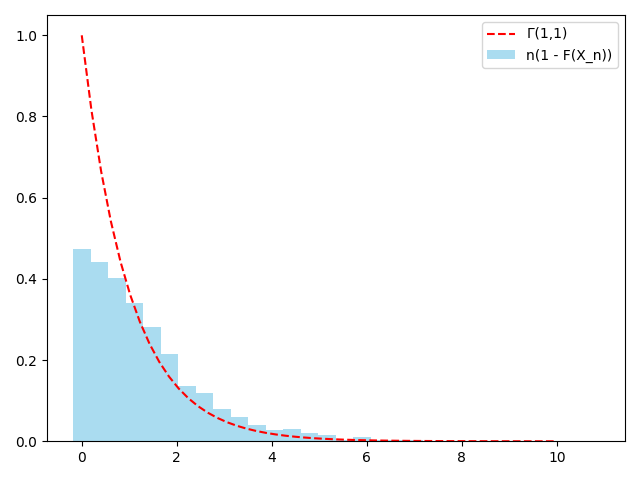
\includegraphics[width=0.5\linewidth]{Python/second-one-one.png}
      % \caption{}
\end{figure}

В итоге можно заключить, что хи-квадрат распределение является частным случаем гамма-распеределения, что видно из гистограмм.



\end{document}